% Options for packages loaded elsewhere
\PassOptionsToPackage{unicode}{hyperref}
\PassOptionsToPackage{hyphens}{url}
%
\documentclass[
  ignorenonframetext,
]{beamer}
\usepackage{pgfpages}
\setbeamertemplate{caption}[numbered]
\setbeamertemplate{caption label separator}{: }
\setbeamercolor{caption name}{fg=normal text.fg}
\beamertemplatenavigationsymbolsempty
% Prevent slide breaks in the middle of a paragraph
\widowpenalties 1 10000
\raggedbottom
\setbeamertemplate{part page}{
  \centering
  \begin{beamercolorbox}[sep=16pt,center]{part title}
    \usebeamerfont{part title}\insertpart\par
  \end{beamercolorbox}
}
\setbeamertemplate{section page}{
  \centering
  \begin{beamercolorbox}[sep=12pt,center]{part title}
    \usebeamerfont{section title}\insertsection\par
  \end{beamercolorbox}
}
\setbeamertemplate{subsection page}{
  \centering
  \begin{beamercolorbox}[sep=8pt,center]{part title}
    \usebeamerfont{subsection title}\insertsubsection\par
  \end{beamercolorbox}
}
\AtBeginPart{
  \frame{\partpage}
}
\AtBeginSection{
  \ifbibliography
  \else
    \frame{\sectionpage}
  \fi
}
\AtBeginSubsection{
  \frame{\subsectionpage}
}
\usepackage{lmodern}
\usepackage{amsmath}
\usepackage{ifxetex,ifluatex}
\ifnum 0\ifxetex 1\fi\ifluatex 1\fi=0 % if pdftex
  \usepackage[T1]{fontenc}
  \usepackage[utf8]{inputenc}
  \usepackage{textcomp} % provide euro and other symbols
  \usepackage{amssymb}
\else % if luatex or xetex
  \usepackage{unicode-math}
  \defaultfontfeatures{Scale=MatchLowercase}
  \defaultfontfeatures[\rmfamily]{Ligatures=TeX,Scale=1}
\fi
% Use upquote if available, for straight quotes in verbatim environments
\IfFileExists{upquote.sty}{\usepackage{upquote}}{}
\IfFileExists{microtype.sty}{% use microtype if available
  \usepackage[]{microtype}
  \UseMicrotypeSet[protrusion]{basicmath} % disable protrusion for tt fonts
}{}
\makeatletter
\@ifundefined{KOMAClassName}{% if non-KOMA class
  \IfFileExists{parskip.sty}{%
    \usepackage{parskip}
  }{% else
    \setlength{\parindent}{0pt}
    \setlength{\parskip}{6pt plus 2pt minus 1pt}}
}{% if KOMA class
  \KOMAoptions{parskip=half}}
\makeatother
\usepackage{xcolor}
\IfFileExists{xurl.sty}{\usepackage{xurl}}{} % add URL line breaks if available
\IfFileExists{bookmark.sty}{\usepackage{bookmark}}{\usepackage{hyperref}}
\hypersetup{
  pdftitle={Charitable Giving, Tax Reform, and Government Efficiency},
  hidelinks,
  pdfcreator={LaTeX via pandoc}}
\urlstyle{same} % disable monospaced font for URLs
\newif\ifbibliography
\usepackage{longtable,booktabs}
\usepackage{calc} % for calculating minipage widths
\usepackage{caption}
% Make caption package work with longtable
\makeatletter
\def\fnum@table{\tablename~\thetable}
\makeatother
\setlength{\emergencystretch}{3em} % prevent overfull lines
\providecommand{\tightlist}{%
  \setlength{\itemsep}{0pt}\setlength{\parskip}{0pt}}
\setcounter{secnumdepth}{-\maxdimen} % remove section numbering
\setbeamertemplate{navigation symbols}{}
\setbeamertemplate{footline}[page number]

\usepackage{bookmark}
\usepackage{booktabs}

\usepackage{xltxtra} 
\usepackage{zxjatype} 
\usepackage[ipa]{zxjafont} 
\ifluatex
  \usepackage{selnolig}  % disable illegal ligatures
\fi

\newlength{\cslhangindent}
\setlength{\cslhangindent}{1.5em}
\newlength{\csllabelwidth}
\setlength{\csllabelwidth}{3em}
\newenvironment{CSLReferences}[3] % #1 hanging-ident, #2 entry spacing
 {% don't indent paragraphs
  \setlength{\parindent}{0pt}
  % turn on hanging indent if param 1 is 1
  \ifodd #1 \everypar{\setlength{\hangindent}{\cslhangindent}}\ignorespaces\fi
  % set entry spacing
  \ifnum #2 > 0
  \setlength{\parskip}{#2\baselineskip}
  \fi
 }%
 {}
\usepackage{calc} % for \widthof, \maxof
\newcommand{\CSLBlock}[1]{#1\hfill\break}
\newcommand{\CSLLeftMargin}[1]{\parbox[t]{\maxof{\widthof{#1}}{\csllabelwidth}}{#1}}
\newcommand{\CSLRightInline}[1]{\parbox[t]{\linewidth}{#1}}
\newcommand{\CSLIndent}[1]{\hspace{\cslhangindent}#1}

\title{Charitable Giving, Tax Reform, and Government Efficiency}
  \author{ Hiroki Kato\(^1\)\and Tsuyoshi Goto\(^2\)\and Yong-Rok Kim\(^3\)}
  \institute{\(^1\)Osaka University\and\(^2\)Chiba University\and\(^3\)Kobe University}
\date{2021/02/03}

\begin{document}
\frame{\titlepage}

\begin{frame}
\end{frame}

\hypertarget{introduction}{%
\section{Introduction}\label{introduction}}

\begin{frame}{Introduction}
\protect\hypertarget{introduction-1}{}
\end{frame}

\hypertarget{data}{%
\section{Data}\label{data}}

\begin{frame}{National Survey of Tax and Benefit (NaSTaB)}
\protect\hypertarget{national-survey-of-tax-and-benefit-nastab}{}
\begin{itemize}
\tightlist
\item
  The Korea Institute of Taxation and Finance implements the financial panel survey to study the tax burden of households and the benefits that households receive from goverment.
\item
  The subjects of this survey are general household and household members living in 15 cities and provinces nationwide.
\item
  This survey is based on a face-to-face interview. If it is difficult for investigators to meet subjects, another family member answers on behalf of him.
\item
  Survey items: Annual taxable income (last year), charitable donations (last year), trust for politicians (5-Likert scale), and other covariates (age, education, gender etc.).
\item
  Survey period: 2008 \textasciitilde{} 2019

  \begin{itemize}
  \tightlist
  \item
    We use survey data after 2013 to focus on tax policy change in 2014.
  \end{itemize}
\end{itemize}
\end{frame}

\begin{frame}{Time Series of Chariable Giving}
\protect\hypertarget{time-series-of-chariable-giving}{}
\begin{figure}

{\centering 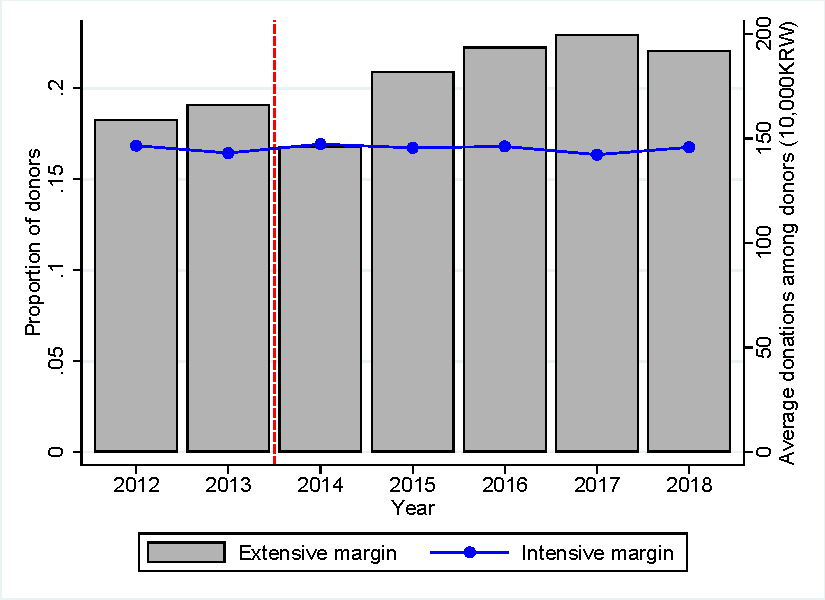
\includegraphics[width=0.9\linewidth]{C:/Users/katoo/Desktop/NASTAB/_assets/SummaryOutcome} 

}

\caption{Proportion of Donors and Average Donations among Donors}\label{fig:unnamed-chunk-1}
\end{figure}
\end{frame}

\begin{frame}{Summary Statistics of Covariates}
\protect\hypertarget{summary-statistics-of-covariates}{}
\begin{table}

\caption{\label{tab:kableSummaryCovariate}Summary Statistics of Covariates}
\centering
\begin{tabular}[t]{lcccc}
\toprule
 & 2012 & 2013 & 2014 & 2015\\
\midrule
Female & 0.51 & 0.51 & 0.52 & 0.52\\
Age & 38.39 & 39.10 & 39.67 & 40.51\\
Annual taxable income & 1699.86 & 1764.04 & 1838.76 & 1872.54\\
University graduate & 0.28 & 0.28 & 0.29 & 0.30\\
High school graduate & 0.30 & 0.30 & 0.31 & 0.31\\
\#.Respondents & 14138 & 13984 & 13787 & 13524\\
\#.Households & 4756 & 4807 & 4819 & 4832\\
\bottomrule
\end{tabular}
\end{table}
\end{frame}

\begin{frame}{Summary Statistics of Covariates (Cont'd)}
\protect\hypertarget{summary-statistics-of-covariates-contd}{}
\begin{table}

\caption{\label{tab:kableSummaryCovariate2}Summary Statistics of Covariates (Continued)}
\centering
\begin{tabular}[t]{lccc}
\toprule
 & 2016 & 2017 & 2018\\
\midrule
Female & 0.52 & 0.52 & 0.52\\
Age & 41.07 & 41.89 & 42.55\\
Annual taxable income & 1906.91 & 1951.55 & 2039.47\\
University graduate & 0.31 & 0.33 & 0.34\\
High school graduate & 0.31 & 0.31 & 0.31\\
\#.Respondents & 13238 & 12963 & 12795\\
\#.Households & 4790 & 4770 & 4765\\
\bottomrule
\end{tabular}
\end{table}
\end{frame}

\begin{frame}{What is Giving Price?}
\protect\hypertarget{what-is-giving-price}{}
Consider allocation between private consumptions (\(x_i\)) and charitable giving (\(g_i\)).
Let \(y_i\) be pre-tax total income.
Then, the budget constraint is

\[
    x_i + g_i = y_i - T_i(y_i, g_i),
\]

where \(T_i\) is tax amount depending on the pre-tax income and charitable giving.
\end{frame}

\begin{frame}{Determination of Tax Amount}
\protect\hypertarget{determination-of-tax-amount}{}
Tax deduction reduces taxable income by giving, that is,

\[
    T_i = \tau(y_i - g_i) \cdot (y_i - g_i),
\]

where \(\tau(\cdot)\) is the marginal income tax rate which is determined by \(y_i - g_i\).

Tax credit reduces tax amount directly, that is,

\[
    T_i = \tau(y_i)\cdot y_i - m g_i,
\]

where \(m \in [0, 1]\) is the tax credit rate.
\end{frame}

\begin{frame}{Derive Giving Price}
\protect\hypertarget{derive-giving-price}{}
Under the tax deduction system, the budget constraint is

\[
    x_i + [1 - \tau(y_i - g_i)]g_i = [1 - \tau(y_i - g_i)] y_i.
\]

Thus, the giving price of tax deduction system is \(p_i^{d} = 1 - \tau(y_i - g_i)\).

Under the tax credit system, the budget constraint is

\[
    x_i + (1 - m) g_i = [1 - \tau(y_i)] y_i.
\]

Thus, the giving price of tax credit system is \(p_i^c = 1 - m\).
\end{frame}

\begin{frame}{Construct Giving Price}
\protect\hypertarget{construct-giving-price}{}
In the South Korea, the tax policy about charitable giving drastically changed in 2014.

\begin{itemize}
\tightlist
\item
  tax deduction (before 2014): \(\text{Price}_i = 1 - \tau(y_i - g_i)\)

  \begin{itemize}
  \tightlist
  \item
    the giving price is endogenous because people can manipulate \(\tau(y_i - g_i)\) using the charitable giving \(g_i\). Since this problem is caused by \emph{last} donations, we use the giving price applying to the \emph{first} donations (\textbf{first price}). The first price is calculate by \(\tau(y_i)\) where \(y_i\) is the annual taxable income reported in the NaSTaB.
  \end{itemize}
\item
  tax credit (after 2014): \(\text{Price}_i = 1 - m\)

  \begin{itemize}
  \tightlist
  \item
    In the South Korea, the tax credit rate determines exogeneity, \(m = 0.15\).
  \end{itemize}
\end{itemize}
\end{frame}

\begin{frame}{Income Distribution and Giving Price}
\protect\hypertarget{income-distribution-and-giving-price}{}
\begin{figure}
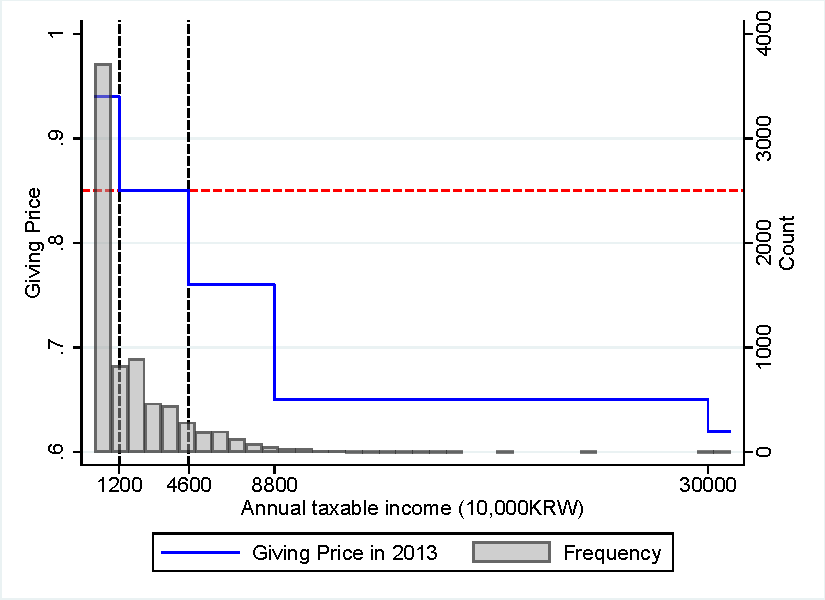
\includegraphics[width=0.9\linewidth]{C:/Users/katoo/Desktop/NASTAB/_assets/SummaryPriceChange} \caption{Income Distribution and Giving Price in 2013}\label{fig:unnamed-chunk-2}
\end{figure}
\end{frame}

\begin{frame}{Time Series of Average Donations By Benefit Group}
\protect\hypertarget{time-series-of-average-donations-by-benefit-group}{}
\begin{figure}
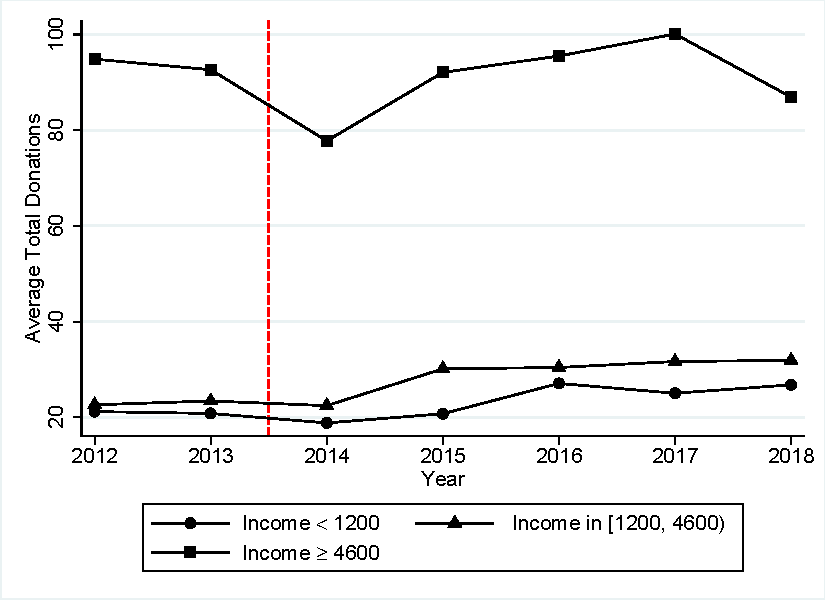
\includegraphics[width=0.9\linewidth]{C:/Users/katoo/Desktop/NASTAB/_assets/AverageDonationsByBenefitGroup} \caption{Time Series of Average Donations by Benefit Group}\label{fig:unnamed-chunk-3}
\end{figure}
\end{frame}

\begin{frame}{Time Series of Extensive Margin by Benfit Group}
\protect\hypertarget{time-series-of-extensive-margin-by-benfit-group}{}
\begin{figure}
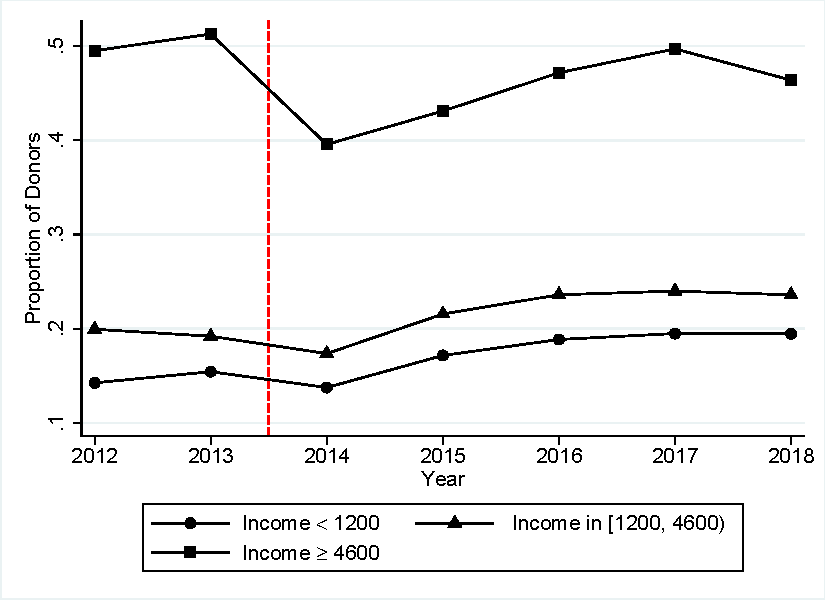
\includegraphics[width=0.9\linewidth]{C:/Users/katoo/Desktop/NASTAB/_assets/ExtensiveByBenefitGroup} \caption{Time Series of Proportion of Donors by Benefit Group}\label{fig:unnamed-chunk-4}
\end{figure}
\end{frame}

\begin{frame}{Time Series of Intensive Margin by Benfit Group}
\protect\hypertarget{time-series-of-intensive-margin-by-benfit-group}{}
\begin{figure}
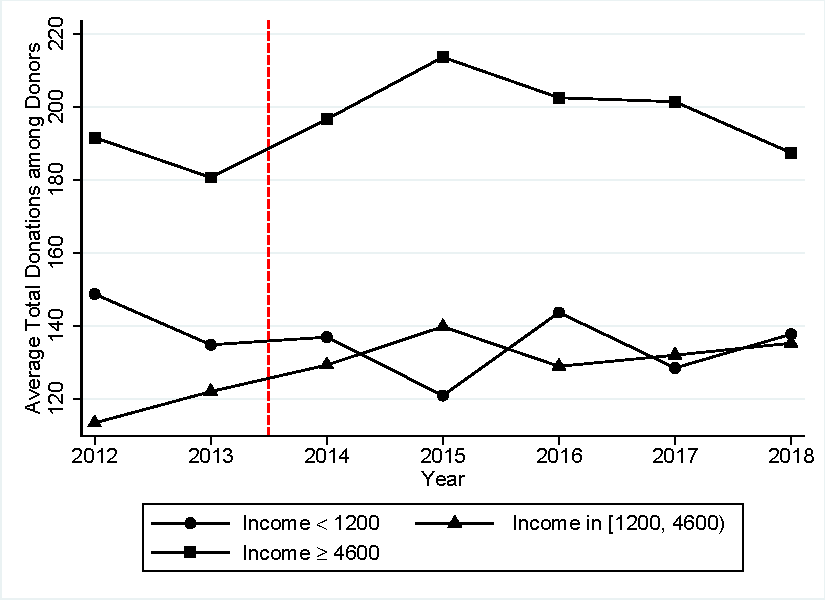
\includegraphics[width=0.9\linewidth]{C:/Users/katoo/Desktop/NASTAB/_assets/IntensiveByBenefitGroup} \caption{Time Series of Average Donations among Donors by Benefit Group}\label{fig:unnamed-chunk-5}
\end{figure}
\end{frame}

\hypertarget{price-elasticity}{%
\section{Price Elasticity}\label{price-elasticity}}

\begin{frame}{Baseline Regressions}
\protect\hypertarget{baseline-regressions}{}
Our baseline regression equation is

\[
    \log(\text{Giving}_{ijt}) = 
    \alpha_i + \beta_1 \log(\text{Price}_{ijt}) + \delta X_{ijt} + \lambda_t + \epsilon_{ijt}.
\]

\begin{itemize}
\tightlist
\item
  \(\log(\text{Giving}_{ijt})\) is logarithm of individual \(i\)'s charitable giving in year \(t\).
\item
  \(\log(\text{Price}_{ijt})\) is logarithm of individual \(i\)'s giving price in year \(t\).
\item
  \(\beta_1\) represents the price elasticity of giving.
\item
  \(\alpha_i\) and \(\lambda_t\) are individual and time fixed effect, respectively.
\end{itemize}
\end{frame}

\begin{frame}{Baseline Regressions: Result}
\protect\hypertarget{baseline-regressions-result}{}
We found the \textbf{price effect} of giving (1\% price increase leads to about 1.1\% giving decrease)

\begin{table}

\caption{\label{tab:kableEstimateElasticity}Baseline Regressions}
\centering
\fontsize{9}{11}\selectfont
\begin{tabular}[t]{lccccc}
\toprule
 & (1) & (2) & (3) & (4) & (5)\\
\midrule
ln(giving price) & -1.071*** & -1.264*** & -1.298*** & -1.117*** & -1.121***\\
 & (0.201) & (0.212) & (0.229) & (0.228) & (0.228)\\
Logged Income & Y & Y & Y & Y & Y\\
Age & N & Y & Y & Y & Y\\
Year X Educ & N & N & Y & Y & Y\\
Year X Gender & N & N & N & Y & Y\\
Resident Area & N & N & N & N & Y\\
N & 54213 & 54213 & 54211 & 54211 & 54211\\
\bottomrule
\end{tabular}
\end{table}
\end{frame}

\begin{frame}{Intensive Margin and Extensive Margin}
\protect\hypertarget{intensive-margin-and-extensive-margin}{}
Let \(D_{ijt}\) be a dummy variable taking 1 if individual \(i\) whose resident area \(j\) in year \(t\) donate in year \(t\)

\begin{itemize}
\tightlist
\item
  Intensive margin: Estiamte \(\beta_1\) where outcome variable is \(\log(\text{Giving}_{ijt})\), using units with \(D_{ijt} = 1\).
\item
  Extensive margin: Estimate \(\beta_1\) where outcome variable is \(D_{ijt}\).

  \begin{itemize}
  \tightlist
  \item
    Extensive-margin price elasticity can be calculated by \(\beta_1/\bar{D}\) where \(\bar{D}\) is the sample mean of \(D_{ijt}\).
  \end{itemize}
\end{itemize}

Covariates in each column corresponds to a column in a previous slide.
\end{frame}

\begin{frame}{Intensive Margin and Extensive Margin: Result}
\protect\hypertarget{intensive-margin-and-extensive-margin-result}{}
\begin{table}

\caption{\label{tab:kableEstimateElasticityIntExt}Intensive-margin and Extensive-Margin Price Elasticity}
\centering
\fontsize{8}{10}\selectfont
\begin{tabular}[t]{lccccc}
\toprule
 & (1) & (2) & (3) & (4) & (5)\\
\midrule
\addlinespace[0.3em]
\multicolumn{6}{l}{\textbf{Intensive Margin}}\\
\hspace{1em}ln(giving price) & -0.593*** & -0.843*** & -1.022*** & -0.887*** & -0.891***\\
\hspace{1em} & (0.202) & (0.212) & (0.231) & (0.242) & (0.243)\\
\hspace{1em} & 11704 & 11704 & 11704 & 11704 & 11704\\
\addlinespace[0.3em]
\multicolumn{6}{l}{\textbf{Extensive Margin}}\\
\hspace{1em}ln(giving price) & -0.258*** & -0.290*** & -0.274*** & -0.238*** & -0.239***\\
\hspace{1em} & (0.046) & (0.048) & (0.052) & (0.052) & (0.052)\\
\hspace{1em}Elasticity & -1.699*** & -1.907*** & -1.807*** & -1.569*** & -1.573***\\
 & (0.301) & (0.316) & (0.341) & (0.341) & (0.341)\\
 & 54213 & 54213 & 54211 & 54211 & 54211\\
\bottomrule
\end{tabular}
\end{table}
\end{frame}

\begin{frame}{Robustness Check}
\protect\hypertarget{robustness-check}{}
\begin{enumerate}
\tightlist
\item
  Income and donations are determined simultaneously
\item
  Effect of presidential transition on donation behavior
\item
  Last price elasticity
\item
  Self-selection of receiving tax benefit
\item
  Transitory and permanent elasticity
\end{enumerate}
\end{frame}

\begin{frame}{Robustness Check 1}
\protect\hypertarget{robustness-check-1}{}
First potential concern: Income and donations are determined simultaneously

\begin{itemize}
\tightlist
\item
  This causes both a change of giving price and a change of an amount of donations
\item
  Gruber and Saez (2002) provided that we should use \(\log(\text{Price}_{ijt}/\text{Price}_{ij(t-k)})\) as an insturment.
\item
  We estimated the model (5) in the previous slide, using the panel IV model for \(k = 1, 2, 3\).

  \begin{itemize}
  \tightlist
  \item
    Note that Alumnia (2020) took a strategy of \(k\)-difference model.
  \end{itemize}
\end{itemize}
\end{frame}

\begin{frame}{Robustness Check 1: Result}
\protect\hypertarget{robustness-check-1-result}{}
\begin{table}

\caption{\label{tab:kablePanelIVEstimateElasticity}Panel IV Regressions}
\centering
\begin{tabular}[t]{lccc}
\toprule
 & k = 1 & k = 2 & k = 3\\
\midrule
ln(giving price) & -1.279*** & -1.155*** & -1.150***\\
 & (0.478) & (0.414) & (0.369)\\
F-stat of IV & 10315.94 & 11506.64 & 11569.61\\
N & 51548 & 49217 & 46399\\
\bottomrule
\end{tabular}
\end{table}
\end{frame}

\begin{frame}{Robustness Check 1: Intensive and Extensive Margin}
\protect\hypertarget{robustness-check-1-intensive-and-extensive-margin}{}
\begin{table}

\caption{\label{tab:kablePanelIVEstimateElasticityIntExt}Intensive- and Extensive-Margin Price Elasticity: Panel IV}
\centering
\fontsize{9}{11}\selectfont
\begin{tabular}[t]{lccc}
\toprule
 & k = 1 & k = 2 & k = 3\\
\midrule
\addlinespace[0.3em]
\multicolumn{4}{l}{\textbf{Intensive Margin}}\\
\hspace{1em}ln(giving price) & -0.0004 & 0.0261 & -0.4378\\
\hspace{1em} & (0.5687) & (0.4410) & (0.3763)\\
\hspace{1em}F-stat of IV & 1679.78 & 2040.66 & 2419.05\\
\hspace{1em}N & 11332 & 10954 & 10451\\
\addlinespace[0.3em]
\multicolumn{4}{l}{\textbf{Extensive Margin}}\\
\hspace{1em}ln(giving price) & -0.3036*** & -0.2944*** & -0.2472***\\
\hspace{1em} & (0.1101) & (0.0934) & (0.0847)\\
\hspace{1em}Elasticity & -2.000*** & -1.939*** & -1.628***\\
\hspace{1em} & (0.725) & (0.615) & (0.558)\\
\hspace{1em}F-stat of IV & 10315.94 & 11506.64 & 11569.61\\
\hspace{1em}N & 51548 & 49217 & 46399\\
\bottomrule
\end{tabular}
\end{table}
\end{frame}

\begin{frame}{Robust Check 2}
\protect\hypertarget{robust-check-2}{}
Second potential concern: The effect of presidential transition on donations

\begin{itemize}
\tightlist
\item
  The presidential transition is one of our major ommited factor to charitable giving.

  \begin{itemize}
  \tightlist
  \item
    In May 2017, South Korea president changed from Park Geun-hye to Moon Jae-in. This presidential transition was due to the impeachment charge against Park Geun-hye. People became distrustful of her due to the shinking of MV Sewol (April 2014).
  \end{itemize}
\item
  To shed light on this concern, we used data in 2013 and 2014 (President was Park Geun-hye in both years), and estimated the model (5) in the previous slide, using the fixed effect model and the panel IV model for \(k = 1, 2, 3\).
\end{itemize}
\end{frame}

\begin{frame}{Robustness Check 2: Result}
\protect\hypertarget{robustness-check-2-result}{}
\begin{table}

\caption{\label{tab:kableShortEstimateElasticity}Results with data in 2013 and 2014}
\centering
\fontsize{9}{11}\selectfont
\begin{tabular}[t]{lcccc}
\toprule
\multicolumn{1}{c}{ } & \multicolumn{1}{c}{FE} & \multicolumn{3}{c}{Panel IV with FE} \\
\cmidrule(l{3pt}r{3pt}){2-2} \cmidrule(l{3pt}r{3pt}){3-5}
 &  & k = 1 & k = 2 & k = 3\\
\midrule
ln(giving price) & -1.466*** & -1.535*** & -1.683*** & -1.151***\\
 & (0.327) & (0.360) & (0.378) & (0.385)\\
F-stat of IV &  & 7420.10 & 4490.74 & 5034.58\\
N & 15134 & 13727 & 12902 & 12420\\
\bottomrule
\end{tabular}
\end{table}
\end{frame}

\begin{frame}{Robustness Check 2: Intensive and Extensive Margin}
\protect\hypertarget{robustness-check-2-intensive-and-extensive-margin}{}
\begin{table}

\caption{\label{tab:kableShortEstimateElasticityIntExt}Intensive- and Extensive-Margin Price Elasticity with Data in 2013 and 2014}
\centering
\fontsize{9}{11}\selectfont
\begin{tabular}[t]{lcccc}
\toprule
\multicolumn{1}{c}{ } & \multicolumn{1}{c}{FE} & \multicolumn{3}{c}{Panel IV with FE} \\
\cmidrule(l{3pt}r{3pt}){2-2} \cmidrule(l{3pt}r{3pt}){3-5}
 &  & k = 1 & k = 2 & k = 3\\
\midrule
\addlinespace[0.3em]
\multicolumn{5}{l}{\textbf{Intensive Margin}}\\
\hspace{1em}ln(giving price) & -0.759** & -0.736* & -0.819** & -0.543\\
\hspace{1em} & (0.344) & (0.418) & (0.404) & (0.371)\\
\hspace{1em}F-stat of IV &  & 1920.08 & 1762.03 & 1706.53\\
\hspace{1em}N & 2938 & 2746 & 2615 & 2512\\
\addlinespace[0.3em]
\multicolumn{5}{l}{\textbf{Extensive Margin}}\\
\hspace{1em}ln(giving price) & -0.332*** & -0.341*** & -0.380*** & -0.291***\\
\hspace{1em} & (0.074) & (0.083) & (0.085) & (0.089)\\
\hspace{1em}Elasticity & -2.186*** & -2.249*** & -2.504*** & -1.920***\\
\hspace{1em} & (0.488) & (0.547) & (0.559) & (0.583)\\
\hspace{1em}F-stat of IV &  & 7420.10 & 4490.74 & 5034.58\\
\hspace{1em}N & 15134 & 13727 & 12902 & 12420\\
\bottomrule
\end{tabular}
\end{table}
\end{frame}

\hypertarget{political-trust-and-price-elasticity}{%
\section{Political Trust and Price Elasticity}\label{political-trust-and-price-elasticity}}

\begin{frame}{Estimation of Trust Index}
\protect\hypertarget{estimation-of-trust-index}{}
The trust for politicans is time-varying variable because it depends on governments' policies.
We make time-invarying trust index using the fixed effect model.

\[
    \text{Trust}_{ijt} = \text{Trustid}_{ij} + c_j \cdot \lambda_t + \lambda_t + \epsilon_{ijt}.
\]

\begin{itemize}
\tightlist
\item
  \(\text{Trust}_{ijt}\): trust for politicians (5-Likert scale)
\item
  \(\text{Trustid}_i\): individual fixed effect (\textbf{Trust index})
\item
  \(c_j \cdot \lambda_t\) captures local governments' policies effect
\item
  \(\lambda_t\) captures the central government policies effect
\end{itemize}
\end{frame}

\begin{frame}{Histrogram of Trust Index}
\protect\hypertarget{histrogram-of-trust-index}{}
\begin{figure}
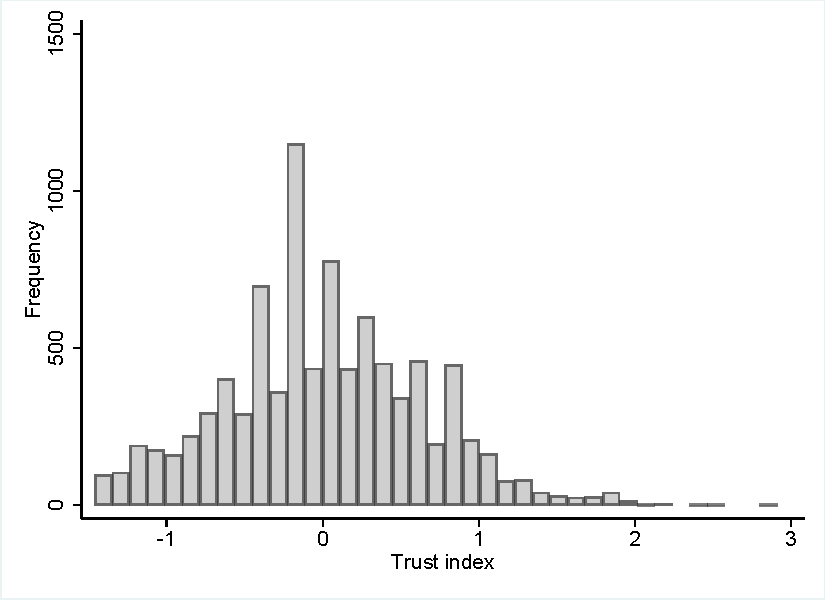
\includegraphics[width=0.9\linewidth]{C:/Users/katoo/Desktop/NASTAB/_assets/HistogramTrustid} \caption{Histogram of Trust Index}\label{fig:unnamed-chunk-6}
\end{figure}
\end{frame}

\begin{frame}{Heterogenous Price Elasticity by Political Trust}
\protect\hypertarget{heterogenous-price-elasticity-by-political-trust}{}
To see the heterogenous price elasticity by political trust,
We estimated the baseline regression model (5) (see Table \ref{tab:kableEstimateElasticity}),
using sample grouped by the trust index.

\begin{itemize}
\tightlist
\item
  Three quantile groups: we divide units \(i\) into the first, second, and third quantile of trust index (1Q, 2Q, and 3Q, respectively).
\end{itemize}
\end{frame}

\begin{frame}{Trust Groups: Descriptive Stats}
\protect\hypertarget{trust-groups-descriptive-stats}{}
\begin{figure}
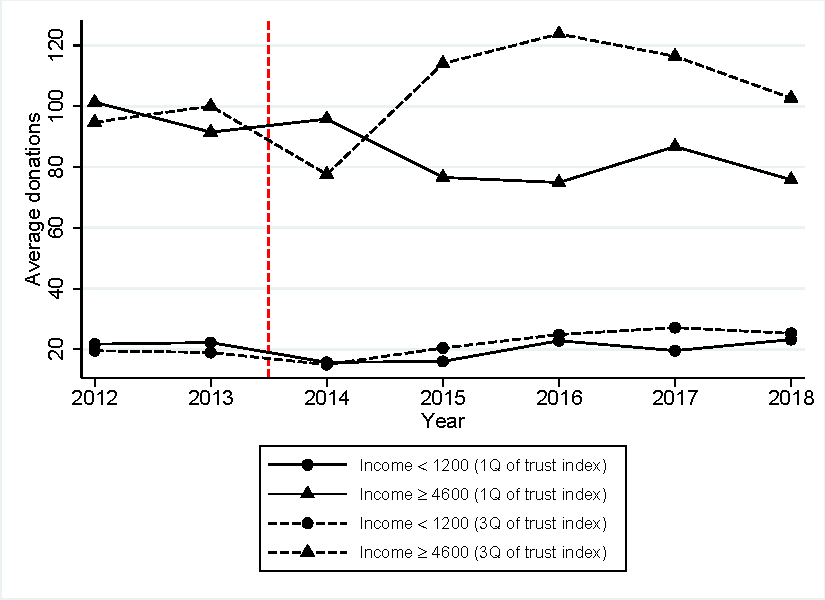
\includegraphics[width=0.9\linewidth]{C:/Users/katoo/Desktop/NASTAB/_assets/SummaryOutcomeByTrustGroup} \caption{Time Series of Average Donations by Subgroup}\label{fig:unnamed-chunk-7}
\end{figure}
\end{frame}

\begin{frame}{Trust Groups: Descriptive Statis (Extensive Margin)}
\protect\hypertarget{trust-groups-descriptive-statis-extensive-margin}{}
\begin{figure}
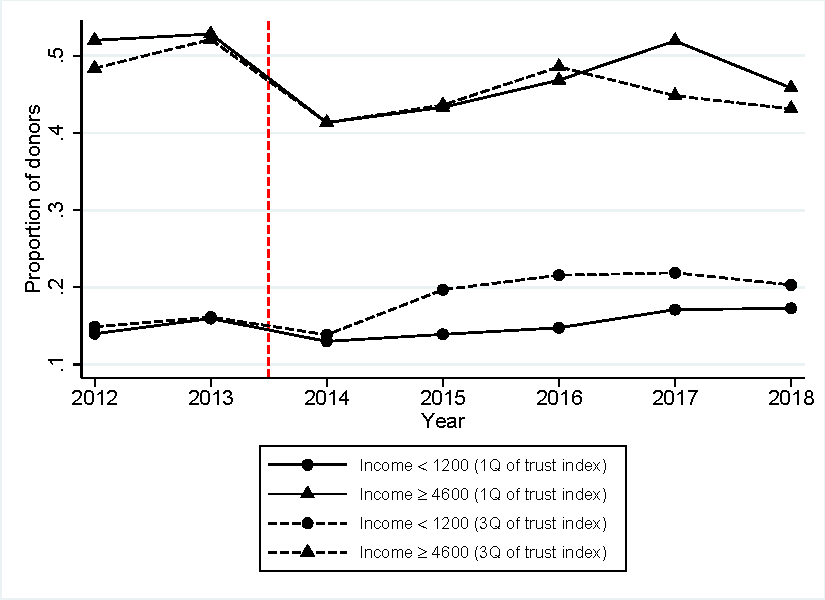
\includegraphics[width=0.9\linewidth]{C:/Users/katoo/Desktop/NASTAB/_assets/SummaryOutcomeExtensiveByTrustGroup} \caption{Time Series of Proportion of Donors by Subgroup}\label{fig:unnamed-chunk-8}
\end{figure}
\end{frame}

\begin{frame}{Trust Groups: Descriptive Stats (Intensive Margin)}
\protect\hypertarget{trust-groups-descriptive-stats-intensive-margin}{}
\begin{figure}
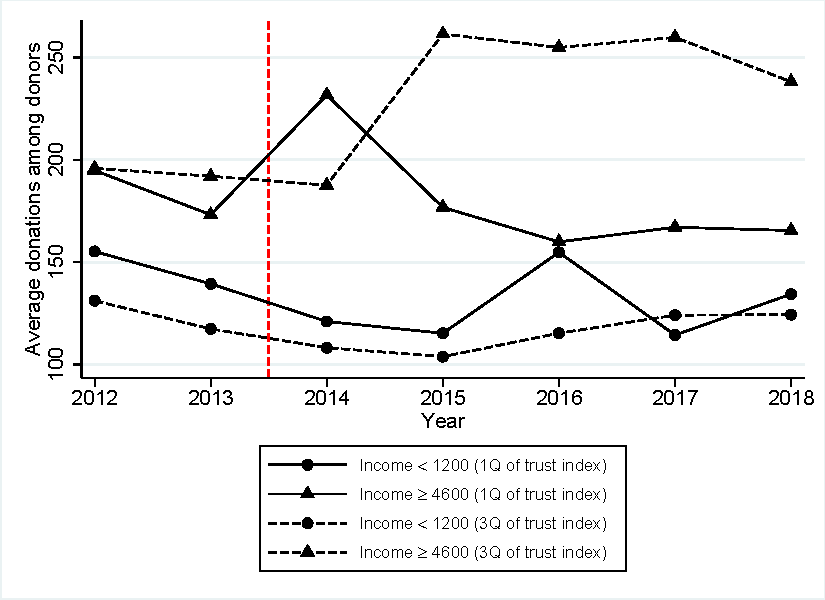
\includegraphics[width=0.9\linewidth]{C:/Users/katoo/Desktop/NASTAB/_assets/SummaryOutcomeIntensiveByTrustGroup} \caption{Time Series of Average Donations among Donors by Subgroup}\label{fig:unnamed-chunk-9}
\end{figure}
\end{frame}

\begin{frame}{Trust Groups: Estimation Result}
\protect\hypertarget{trust-groups-estimation-result}{}
\begin{table}

\caption{\label{tab:kableEstimateElasticityIntExtByTrustGroup3}Price Elasticity by Three Quantile Trust Groups}
\centering
\fontsize{8}{10}\selectfont
\begin{tabular}[t]{lccc}
\toprule
 & 1Q & 2Q & 3Q\\
\midrule
\addlinespace[0.3em]
\multicolumn{4}{l}{\textbf{Overall}}\\
\hspace{1em}ln(giving price) & -0.496 & -1.635*** & -1.157***\\
\hspace{1em} & (0.398) & (0.391) & (0.410)\\
\hspace{1em}N & 17421 & 16810 & \vphantom{1} 17075\\
\addlinespace[0.3em]
\multicolumn{4}{l}{\textbf{Intensive Margin}}\\
\hspace{1em}ln(giving price) & -0.997** & -0.980** & -0.208\\
\hspace{1em} & (0.408) & (0.398) & (0.450)\\
\hspace{1em}N & 3516 & 3959 & 3917\\
\addlinespace[0.3em]
\multicolumn{4}{l}{\textbf{Extensive Margin}}\\
\hspace{1em}ln(giving price) & -0.131 & -0.327*** & -0.244***\\
\hspace{1em} & (0.089) & (0.090) & (0.093)\\
\hspace{1em}Elasticity & -0.722 & -1.571*** & -1.088***\\
\hspace{1em} & (0.487) & (0.433) & (0.416)\\
\hspace{1em}N & 17421 & 16810 & 17075\\
\bottomrule
\end{tabular}
\end{table}
\end{frame}

\begin{frame}{Robustness Check}
\protect\hypertarget{robustness-check-2}{}
\begin{enumerate}
\tightlist
\item
  Effect of presidential transition on trust index
\item
  Effect of presidential transition on donation behavior
\item
  Income and donations are determined simultaneously
\item
  Last price elasticity
\item
  Self-selection of receiving tax benefit
\item
  Transitory and permanent elasticity
\end{enumerate}
\end{frame}

\begin{frame}{Robustness Check 1: Presidential Transition Effect on Trust}
\protect\hypertarget{robustness-check-1-presidential-transition-effect-on-trust}{}
\begin{itemize}
\tightlist
\item
  Even though we control time fixed effect when estimating the trust index, we may not rule out the effect of presidential transition on it perfectly.
\item
  To check this point, we repeat estimate the same model using either data in 2015 and 2016 (Park's trust index) or in 2017 and 2018 (Moon's trust index), and obtain the president-specific trust indexs. After that, we test whether the average individual difference b/w these two indexs is statistically different from zero (pair-wise t-test).
\item
  As a result, the average individual difference is -0.008 (s.e. = 0.01). This difference is not statistically different from zero (p-value = 0.446).
\end{itemize}
\end{frame}

\begin{frame}{Robustness Check 2}
\protect\hypertarget{robustness-check-2-1}{}
We check the following two potential concerns

\begin{itemize}
\tightlist
\item
  Presidential transition effect on donation behavior
\item
  Income and donations are determined simultaneously
\end{itemize}

To address these problems, we estimate the FE model and Panel IV model with FE where instrument is \(\log(\text{Price}_{ijt}/\text{Price}_{ij(t-k)})\) for \(k = 1, 2, 3\), using data in 2013 and 2014.

Note that f-statistics of IV is greater than 1000 when we estimate overall elasticity and extensive-margin elasticity, and greater than 400 when we estimate the intensive-margin elasticity.
\end{frame}

\begin{frame}{Robustness Check 2: Result}
\protect\hypertarget{robustness-check-2-result-1}{}
\begin{table}

\caption{\label{tab:tabShortEstimateElasticityByTrustGroup3}Robustness Check of Heterogenous Price Elasiticity by Political Trust}
\centering
\fontsize{8}{10}\selectfont
\begin{tabular}[t]{lccc}
\toprule
 & 1Q & 2Q & 3Q\\
\midrule
\addlinespace[0.3em]
\multicolumn{4}{l}{\textbf{FE Model}}\\
\hspace{1em}ln(giving price) & -0.485 & -2.901*** & -1.164*\\
\hspace{1em} & (0.564) & (0.563) & (0.623)\\
\hspace{1em}N & 4713 & 4489 & 4586\\
\addlinespace[0.3em]
\multicolumn{4}{l}{\textbf{Panel IV (k = 1)}}\\
\hspace{1em}ln(giving price) & -0.347 & -3.307*** & -1.242*\\
\hspace{1em} & (0.639) & (0.602) & (0.656)\\
\hspace{1em}N & 4337 & 4109 & 4190\\
\addlinespace[0.3em]
\multicolumn{4}{l}{\textbf{Panel IV (k = 2)}}\\
\hspace{1em}ln(giving price) & -0.617 & -3.314*** & -1.204*\\
\hspace{1em} & (0.627) & (0.689) & (0.702)\\
\hspace{1em}N & 4100 & 3839 & 3975\\
\addlinespace[0.3em]
\multicolumn{4}{l}{\textbf{Panel IV (k = 3)}}\\
\hspace{1em}ln(giving price) & -0.230 & -2.536*** & -0.807\\
\hspace{1em} & (0.684) & (0.673) & (0.691)\\
\hspace{1em}N & 3947 & 3700 & 3832\\
\bottomrule
\end{tabular}
\end{table}
\end{frame}

\begin{frame}{Robustness Check 2: Result (Extensive Margin)}
\protect\hypertarget{robustness-check-2-result-extensive-margin}{}
\begin{table}

\caption{\label{tab:tabShortEstimateElasticityExtensiveByTrustGroup3}Robustness Check of Heterogenous Extensive-Margin Price Elasiticity by Political Trust}
\centering
\fontsize{8}{10}\selectfont
\begin{tabular}[t]{lccc}
\toprule
 & 1Q & 2Q & 3Q\\
\midrule
\addlinespace[0.3em]
\multicolumn{4}{l}{\textbf{FE Model}}\\
\hspace{1em}Implied Elasticity & -0.834 & -3.347*** & -1.386*\\
\hspace{1em} & (0.728) & (0.672) & (0.774)\\
\hspace{1em}N & 4713 & 4489 & 4586\\
\addlinespace[0.3em]
\multicolumn{4}{l}{\textbf{Panel IV (k = 1)}}\\
\hspace{1em}Implied Elasticity & -0.438 & -3.880*** & -1.658*\\
\hspace{1em} & (0.816) & (0.732) & (0.846)\\
\hspace{1em}N & 4337 & 4109 & 4190\\
\addlinespace[0.3em]
\multicolumn{4}{l}{\textbf{Panel IV (k = 2)}}\\
\hspace{1em}Implied Elasticity & -1.082 & -3.864*** & -1.223\\
\hspace{1em} & (0.805) & (0.797) & (0.878)\\
\hspace{1em}N & 4100 & 3839 & 3975\\
\addlinespace[0.3em]
\multicolumn{4}{l}{\textbf{Panel IV (k = 3)}}\\
\hspace{1em}Implied Elasticity & -0.852 & -3.176*** & -0.850\\
\hspace{1em} & (0.881) & (0.806) & (0.893)\\
\hspace{1em}N & 3947 & 3700 & 3832\\
\bottomrule
\end{tabular}
\end{table}
\end{frame}

\begin{frame}{Robustness Check 2: Result (Intensive Margin)}
\protect\hypertarget{robustness-check-2-result-intensive-margin}{}
\begin{table}

\caption{\label{tab:tabShortEstimateElasticityIntensiveByTrustGroup3}Robustness Check of Heterogenous Intenstive-Margin Price Elasiticity by Political Trust}
\centering
\fontsize{8}{10}\selectfont
\begin{tabular}[t]{lccc}
\toprule
 & 1Q & 2Q & 3Q\\
\midrule
\addlinespace[0.3em]
\multicolumn{4}{l}{\textbf{FE Model}}\\
\hspace{1em}ln(giving price) & -0.946* & -0.969* & -0.622\\
\hspace{1em} & (0.540) & (0.575) & (0.673)\\
\hspace{1em}N & 904 & 958 & 931\\
\addlinespace[0.3em]
\multicolumn{4}{l}{\textbf{Panel IV (k = 1)}}\\
\hspace{1em}ln(giving price) & -1.408** & -0.687 & -0.396\\
\hspace{1em} & (0.636) & (0.710) & (0.841)\\
\hspace{1em}N & 847 & 898 & 881\\
\addlinespace[0.3em]
\multicolumn{4}{l}{\textbf{Panel IV (k = 2)}}\\
\hspace{1em}ln(giving price) & -1.117* & -0.912 & -0.696\\
\hspace{1em} & (0.651) & (0.657) & (0.787)\\
\hspace{1em}N & 812 & 850 & 844\\
\addlinespace[0.3em]
\multicolumn{4}{l}{\textbf{Panel IV (k = 3)}}\\
\hspace{1em}ln(giving price) & -0.640 & -0.611 & -0.327\\
\hspace{1em} & (0.609) & (0.596) & (0.698)\\
\hspace{1em}N & 777 & 819 & 816\\
\bottomrule
\end{tabular}
\end{table}
\end{frame}

\hypertarget{governement-efficient-and-price-elasticity}{%
\section{Governement Efficient and Price Elasticity}\label{governement-efficient-and-price-elasticity}}

\begin{frame}{Government Efficiency}
\protect\hypertarget{government-efficiency}{}
From the 2015 survey,
NaSTaB asks the current and ideal balance between tax burden and welfare size.

These variables provide us to investigate the relationship between price elasticity and govenrment's efficiency
more directly.

Thus, we did same excercise, using the current balance bewteen tax burden and welfare size.
\end{frame}

\begin{frame}{Construct Efficient Index}
\protect\hypertarget{construct-efficient-index}{}
Questionnaire of tax-welfare balance index is

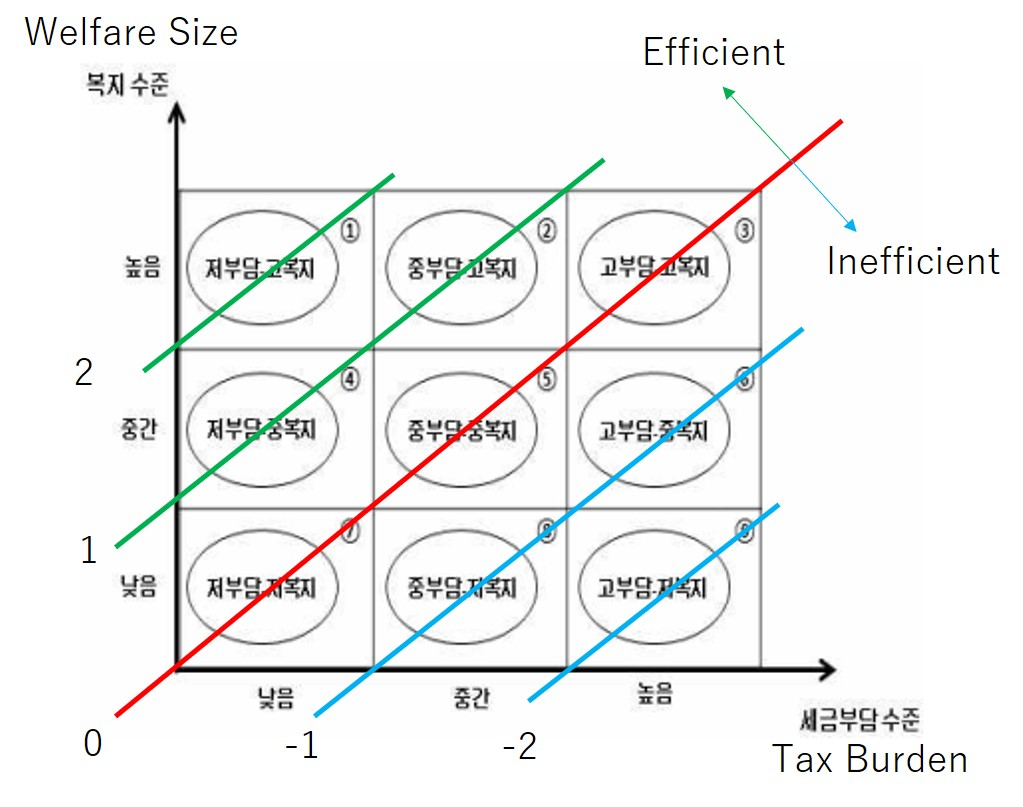
\includegraphics[width=0.5\textwidth,height=\textheight]{_assets/BalanceQuestion.jpg}

To rule out government's policies, we use individual fixed effect as the \textbf{efficient index}
\end{frame}

\begin{frame}{Histrogram of Efficient Index}
\protect\hypertarget{histrogram-of-efficient-index}{}
\begin{figure}
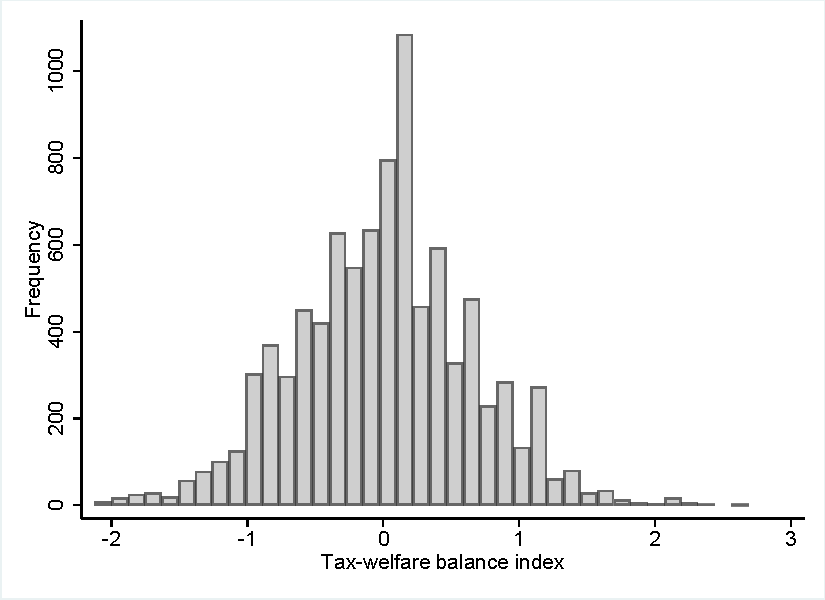
\includegraphics[width=0.9\linewidth]{C:/Users/katoo/Desktop/NASTAB/_assets/HistogramBalanceid} \caption{Histogram of Efficient Index}\label{fig:unnamed-chunk-10}
\end{figure}
\end{frame}

\begin{frame}{Heterogenous Price Elasticity by Governement Efficiency}
\protect\hypertarget{heterogenous-price-elasticity-by-governement-efficiency}{}
To see the heterogenous price elasticity by efficient index,
We estimated the baseline regression model (5) (see Table \ref{tab:kableEstimateElasticity}),
using sample grouped by the efficient index.

\begin{itemize}
\tightlist
\item
  Three quantile groups: we divide units \(i\) into the first, second, and third quantile of efficient index (1Q, 2Q, and 3Q, respectively).
\end{itemize}
\end{frame}

\begin{frame}{Efficient Groups: Descriptive Stats}
\protect\hypertarget{efficient-groups-descriptive-stats}{}
\begin{figure}
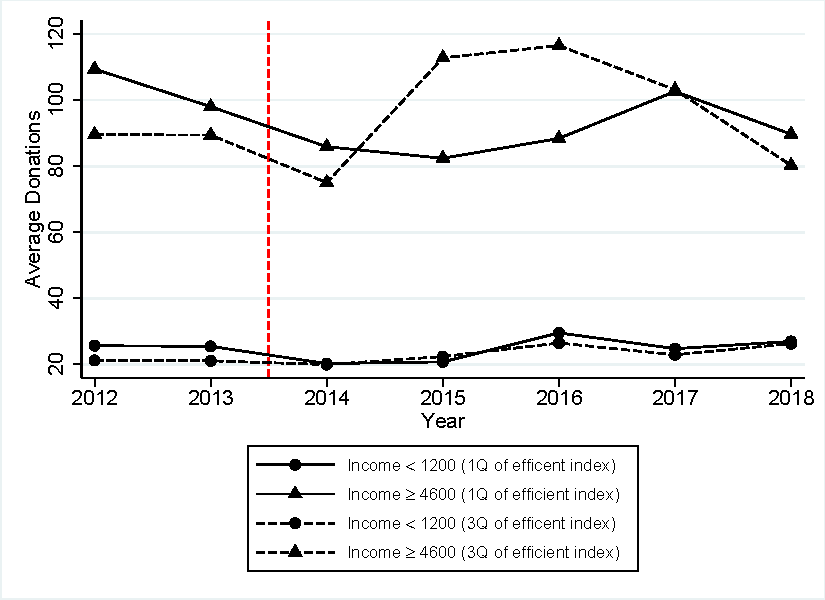
\includegraphics[width=0.9\linewidth]{C:/Users/katoo/Desktop/NASTAB/_assets/SummaryOutcomeByEfficientGroup3} \caption{Time Series of Average Donations by Subgroup}\label{fig:unnamed-chunk-11}
\end{figure}
\end{frame}

\begin{frame}{Efficient Groups: Descriptive Statis (Extensive Margin)}
\protect\hypertarget{efficient-groups-descriptive-statis-extensive-margin}{}
\begin{figure}
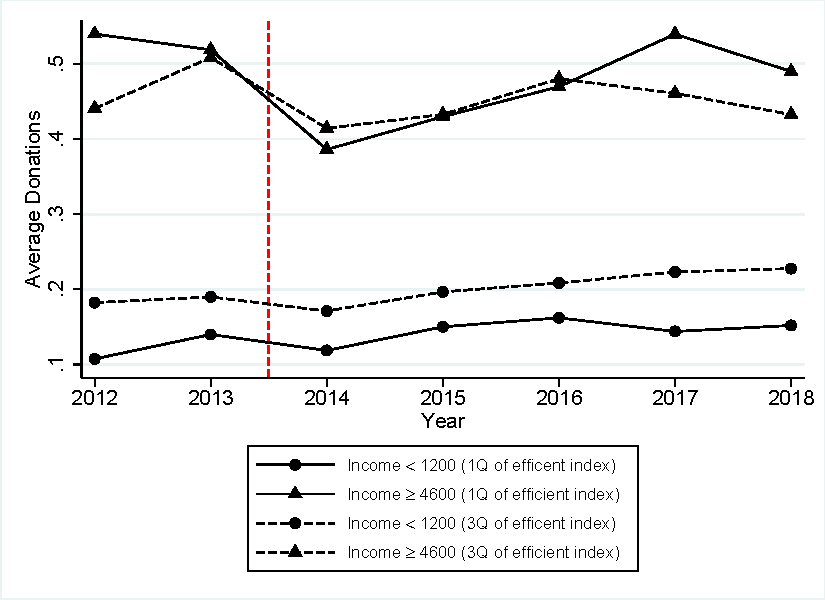
\includegraphics[width=0.9\linewidth]{C:/Users/katoo/Desktop/NASTAB/_assets/SummaryOutcomeExtensiveByEfficientGroup3} \caption{Time Series of Proportion of Donors by Subgroup}\label{fig:unnamed-chunk-12}
\end{figure}
\end{frame}

\begin{frame}{Efficient Groups: Descriptive Stats (Intensive Margin)}
\protect\hypertarget{efficient-groups-descriptive-stats-intensive-margin}{}
\begin{figure}
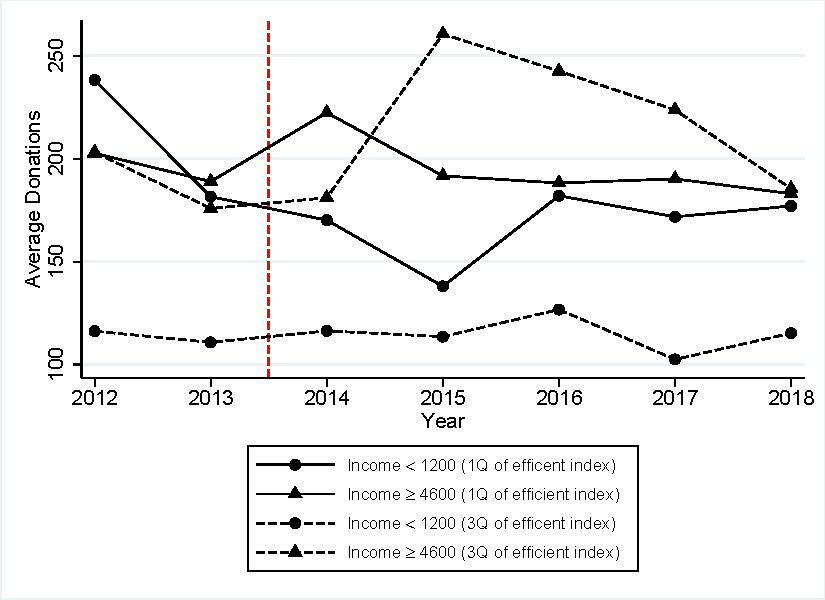
\includegraphics[width=0.9\linewidth]{C:/Users/katoo/Desktop/NASTAB/_assets/SummaryOutcomeIntensiveByEfficientGroup3} \caption{Time Series of Average Donations among Donors by Subgroup}\label{fig:unnamed-chunk-13}
\end{figure}
\end{frame}

\begin{frame}{Efficient Groups: Estimation Results}
\protect\hypertarget{efficient-groups-estimation-results}{}
\begin{table}

\caption{\label{tab:kableEstimateElasticityByEfficientGroup3}Price Elasticity by Three Quantile Efficient Groups}
\centering
\fontsize{8}{10}\selectfont
\begin{tabular}[t]{lccc}
\toprule
 & 1Q & 2Q & 3Q\\
\midrule
\addlinespace[0.3em]
\multicolumn{4}{l}{\textbf{Overall}}\\
\hspace{1em}ln(giving price) & -1.321*** & -0.844** & -0.929**\\
\hspace{1em} & (0.388) & (0.404) & (0.404)\\
\hspace{1em}N & 17119 & 16662 & \vphantom{1} 17525\\
\addlinespace[0.3em]
\multicolumn{4}{l}{\textbf{Intensive Margin}}\\
\hspace{1em}ln(giving price) & -0.792** & -0.360 & -1.111**\\
\hspace{1em} & (0.383) & (0.423) & (0.497)\\
\hspace{1em}N & 3696 & 3591 & 4105\\
\addlinespace[0.3em]
\multicolumn{4}{l}{\textbf{Extensive Margin}}\\
\hspace{1em}ln(giving price) & -0.276*** & -0.225** & -0.174*\\
\hspace{1em} & (0.087) & (0.094) & (0.091)\\
\hspace{1em}Elasticity & -1.380*** & -1.115** & -0.787*\\
\hspace{1em} & (0.435) & (0.466) & (0.412)\\
\hspace{1em}N & 17119 & 16662 & 17525\\
\bottomrule
\end{tabular}
\end{table}
\end{frame}

\begin{frame}{Robustness Check}
\protect\hypertarget{robustness-check-3}{}
\begin{enumerate}
\tightlist
\item
  Efficient index captures both government efficiency on concerns about budget deficits
\item
  Effect of presidential transition on efficient index
\item
  Effect of presidential transition on donation behavior
\item
  Income and donations are determined simultaneously
\item
  Last price elasticity
\item
  Self-selection of receiving tax benefit
\item
  Transitory and permanent elasticity
\end{enumerate}
\end{frame}

\begin{frame}{Robustness Check 1}
\protect\hypertarget{robustness-check-1-1}{}
\begin{itemize}
\tightlist
\item
  Efficient index may capture both government efficiency on concerns about budget deficits

  \begin{itemize}
  \tightlist
  \item
    NASTAB asks respondents to answer the ideal balance b/w tax burdern and welfare size.
  \item
    We constructed the \textbf{ideal} efficient index, using the FE model to estimate the efficient index.
  \item
    We droped units with the ideal efficient index is less than 0 from each quantile group and repeated the same excercise.
  \item
    This is because respondents whose the ideal efficient index is less than 0 think governments should try to avoid budget deficits (high tax, low welfare).
  \end{itemize}
\item
  Presidential transition effect on perceived efficiency

  \begin{itemize}
  \tightlist
  \item
    We constructed president-specific (ideal) efficient index and implemented the pair-wise t-test.
  \item
    As a result, average difference of these two indexs are not statistically siginificant zero.
  \end{itemize}
\end{itemize}
\end{frame}

\begin{frame}{Robustness Check 1: Estimation Results}
\protect\hypertarget{robustness-check-1-estimation-results}{}
\begin{table}

\caption{\label{tab:kableEstimateElasticityByPositiveEfficientGroup3}Heterogenous Price Elasticity by Efficiency Using Units with Ideal Efficient Index > 0}
\centering
\fontsize{8}{10}\selectfont
\begin{tabular}[t]{lccc}
\toprule
 & 1Q & 2Q & 3Q\\
\midrule
\addlinespace[0.3em]
\multicolumn{4}{l}{\textbf{Overall}}\\
\hspace{1em}ln(giving price) & -1.996*** & -1.122* & -0.063\\
\hspace{1em} & (0.648) & (0.597) & (0.488)\\
\hspace{1em}N & 7527 & 6900 & \vphantom{1} 9339\\
\addlinespace[0.3em]
\multicolumn{4}{l}{\textbf{Intensive Margin}}\\
\hspace{1em}ln(giving price) & -1.138* & -0.900 & -0.952\\
\hspace{1em} & (0.640) & (0.652) & (0.741)\\
\hspace{1em}N & 1541 & 1474 & 2023\\
\addlinespace[0.3em]
\multicolumn{4}{l}{\textbf{Extensive Margin}}\\
\hspace{1em}ln(giving price) & -0.317** & -0.220 & 0.014\\
\hspace{1em} & (0.136) & (0.137) & (0.119)\\
\hspace{1em}Elasticity & -1.582** & -1.091 & 0.062\\
\hspace{1em} & (0.681) & (0.679) & (0.537)\\
\hspace{1em}N & 7527 & 6900 & 9339\\
\bottomrule
\end{tabular}
\end{table}
\end{frame}

\begin{frame}{Robustness Check 2}
\protect\hypertarget{robustness-check-2-2}{}
We check the following two potential concerns

\begin{itemize}
\tightlist
\item
  Presidential transition effect on donation behavior
\item
  Income and donations are determined simultaneously
\end{itemize}

To address these problems, we estimated the FE model and Panel IV model with FE where instrument is \(\log(\text{Price}_{ijt}/\text{Price}_{ij(t-k)})\) for \(k = 1, 2, 3\), using data in 2013 and 2014.
Moreover, we droped units with the ideal efficient index \textless{} 0 from each quantile group.

Note that f-statistics of IV is greater than 500 when we estimate overall elasticity and extensive-margin elasticity, and greater than 100 when we estimate the intensive-margin elasticity.
\end{frame}

\begin{frame}{Robustness Check 2: Result}
\protect\hypertarget{robustness-check-2-result-2}{}
\begin{table}

\caption{\label{tab:tabShortEstimateElasticityByEfficientGroup3}Robustness Check of Heterogenous Price Elasiticity by Government Efficiency}
\centering
\fontsize{8}{10}\selectfont
\begin{tabular}[t]{lccc}
\toprule
 & 1Q & 2Q & 3Q\\
\midrule
\addlinespace[0.3em]
\multicolumn{4}{l}{\textbf{FE Model}}\\
\hspace{1em}ln(giving price) & -1.989** & -1.047 & -1.881**\\
\hspace{1em} & (0.913) & (1.078) & (0.835)\\
\hspace{1em}N & 2021 & 1841 & 2504\\
\addlinespace[0.3em]
\multicolumn{4}{l}{\textbf{Panel IV (k = 1)}}\\
\hspace{1em}ln(giving price) & -1.881* & -1.093 & -2.189**\\
\hspace{1em} & (0.992) & (1.272) & (0.851)\\
\hspace{1em}N & 1842 & 1689 & 2292\\
\addlinespace[0.3em]
\multicolumn{4}{l}{\textbf{Panel IV (k = 2)}}\\
\hspace{1em}ln(giving price) & -1.958* & -1.594 & -1.684\\
\hspace{1em} & (1.101) & (1.212) & (1.024)\\
\hspace{1em}N & 1723 & 1582 & 2174\\
\addlinespace[0.3em]
\multicolumn{4}{l}{\textbf{Panel IV (k = 3)}}\\
\hspace{1em}ln(giving price) & -1.608 & -0.317 & -1.544\\
\hspace{1em} & (1.079) & (1.219) & (0.999)\\
\hspace{1em}N & 1645 & 1529 & 2096\\
\bottomrule
\end{tabular}
\end{table}
\end{frame}

\begin{frame}{Robustness Check 2: Result (Extensive Margin)}
\protect\hypertarget{robustness-check-2-result-extensive-margin-1}{}
\begin{table}

\caption{\label{tab:tabShortEstimateElasticityExtensiveByEfficientGroup3}Robustness Check of Heterogenous Extensive-Margin Price Elasiticity by Government Efficiency}
\centering
\fontsize{8}{10}\selectfont
\begin{tabular}[t]{lccc}
\toprule
 & 1Q & 2Q & 3Q\\
\midrule
\addlinespace[0.3em]
\multicolumn{4}{l}{\textbf{FE Model}}\\
\hspace{1em}Implied Elasticity & -1.558 & -0.649 & -2.453**\\
\hspace{1em} & (1.119) & (1.326) & (1.147)\\
\hspace{1em}N & 2021 & 1841 & 2504\\
\addlinespace[0.3em]
\multicolumn{4}{l}{\textbf{Panel IV (k = 1)}}\\
\hspace{1em}Implied Elasticity & -1.345 & -0.517 & -2.934**\\
\hspace{1em} & (1.255) & (1.612) & (1.180)\\
\hspace{1em}N & 1842 & 1689 & 2292\\
\addlinespace[0.3em]
\multicolumn{4}{l}{\textbf{Panel IV (k = 2)}}\\
\hspace{1em}Implied Elasticity & -1.396 & -1.557 & -1.998\\
\hspace{1em} & (1.264) & (1.486) & (1.439)\\
\hspace{1em}N & 1723 & 1582 & 2174\\
\addlinespace[0.3em]
\multicolumn{4}{l}{\textbf{Panel IV (k = 3)}}\\
\hspace{1em}Implied Elasticity & -1.056 & -0.460 & -1.795\\
\hspace{1em} & (1.262) & (1.477) & (1.355)\\
\hspace{1em}N & 1645 & 1529 & 2096\\
\bottomrule
\end{tabular}
\end{table}
\end{frame}

\begin{frame}{Robustness Check 2: Result (Intensive Margin)}
\protect\hypertarget{robustness-check-2-result-intensive-margin-1}{}
\begin{table}

\caption{\label{tab:tabShortEstimateElasticityIntensiveByEfficientGroup3}Robustness Check of Heterogenous Intenstive-Margin Price Elasiticity by Government Efficiency}
\centering
\fontsize{8}{10}\selectfont
\begin{tabular}[t]{lccc}
\toprule
 & 1Q & 2Q & 3Q\\
\midrule
\addlinespace[0.3em]
\multicolumn{4}{l}{\textbf{FE Model}}\\
\hspace{1em}ln(giving price) & -0.753 & -2.301* & -1.362\\
\hspace{1em} & (0.848) & (1.310) & (0.956)\\
\hspace{1em}N & 404 & 361 & 479\\
\addlinespace[0.3em]
\multicolumn{4}{l}{\textbf{Panel IV (k = 1)}}\\
\hspace{1em}ln(giving price) & -0.749 & -3.220* & -1.471\\
\hspace{1em} & (1.088) & (1.812) & (1.013)\\
\hspace{1em}N & 380 & 340 & 449\\
\addlinespace[0.3em]
\multicolumn{4}{l}{\textbf{Panel IV (k = 2)}}\\
\hspace{1em}ln(giving price) & -0.770 & -1.216 & -0.771\\
\hspace{1em} & (0.997) & (1.504) & (0.966)\\
\hspace{1em}N & 357 & 322 & 433\\
\addlinespace[0.3em]
\multicolumn{4}{l}{\textbf{Panel IV (k = 3)}}\\
\hspace{1em}ln(giving price) & 0.573 & -0.691 & -1.472\\
\hspace{1em} & (1.117) & (1.088) & (0.991)\\
\hspace{1em}N & 337 & 307 & 414\\
\bottomrule
\end{tabular}
\end{table}
\end{frame}

\begin{frame}{References}
\protect\hypertarget{references}{}
\hypertarget{refs}{}
\begin{CSLReferences}{1}{0}
\leavevmode\hypertarget{ref-Bursztyn2017}{}%
Bursztyn, L., Jensen, R., 2017. Social image and economic behavior in the field: Identifying, understanding, and shaping social pressure. Annual Review of Economics 9, 131--153. doi:\href{https://doi.org/10.1146/annurev-economics-063016-103625}{10.1146/annurev-economics-063016-103625}

\end{CSLReferences}
\end{frame}

\end{document}
